\RequirePackage[l2tabu, orthodox]{nag}
\documentclass[12pt]{article}

\usepackage{amssymb,amsmath,verbatim,graphicx,microtype,units,booktabs}
\usepackage[margin=10pt, font=small, labelfont=bf, labelsep=endash]{caption}
\usepackage[colorlinks=true, pdfborder={0 0 0}]{hyperref}
\usepackage[utf8]{inputenc}

\usepackage{xcolor}
\newcommand{\shellcmd}[1]{\texttt{\colorbox{gray!30}{#1}}}
\newcommand{\todo}[2]{\textbf{\colorbox{red!50}{#1}}{\footnote{#2}}}
\newcommand{\br}{\multicolumn{2}{c}{} \\}
\newcommand{\gray}{\rowcolor[gray]{.9}}

\usepackage[left=1.15in, right=1.15in]{geometry}
\usepackage{titleps}
\newpagestyle{main}{
    \setheadrule{.4pt}
    \sethead{\sectiontitle}
            {}
            {Illya Starikov}
}
\pagestyle{main}

\usepackage{siunitx}
\begin{document}
\title{Lab \#1: Laboratory Equipment}
\date{January 25, 2016}
\author{Illya Starikov}
\maketitle


\section{Objective}
To familiarize self with lab equipment, namely the DC Power Supply, Function Generator, Frequency Counter/Timer, Digital Multimeter, and Mixed Signal Oscilloscope.

\section{Equipment Used}
\begin{itemize}
\item DC Power Supply
\item Function Generator
\item Frequency Counter/Timer
\item Digital Multimeter
\item Mixed Signal Oscilloscope
\end{itemize}

\section{Procedures}
\begin{enumerate}
\item Generate a square wave with an amplitude of \SI{3}{\volt} and frequency of \SI{900}{\hertz}.
    \begin{itemize}
    \item Offset DC by \SI{2}{\volt}.
    \end{itemize}
\item Generate 3 signals:
    \begin{itemize}
    \item \SI{1}{\kilo\hertz}
    \item \SI{10}{\kilo\hertz}
    \item \SI{50}{\kilo\hertz}
    \end{itemize}
\item Generate \SI{7}{\volt} DC, measuring with the Digital Multimeter.
\item Follow the steps of category 5.
\end{enumerate}

\section{Conclusion and Results}
\subsection{Function Generator}
% \noindent\makebox[\textwidth]{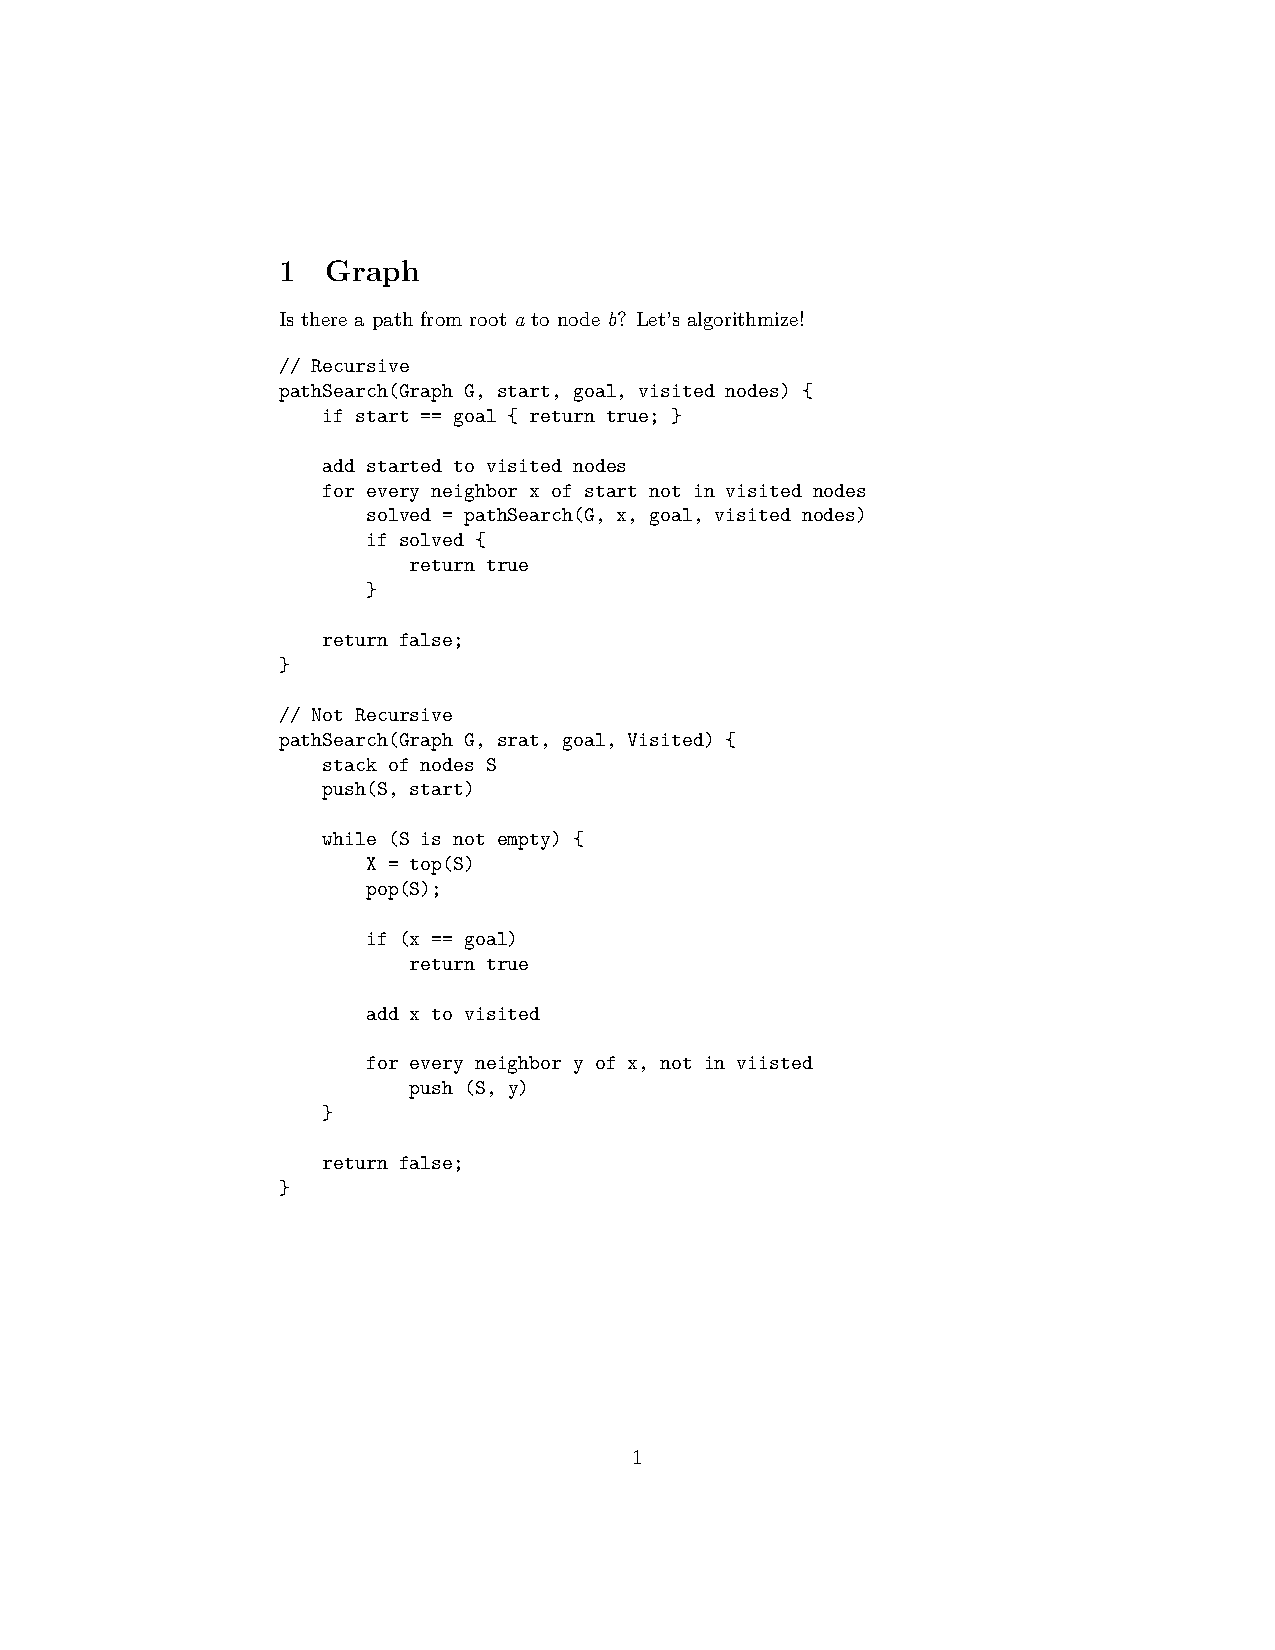
\includegraphics[width=\paperwidth]{Graph}}

\subsection{Frequency Counter/Timer}
\begin{center}
\begin{tabular}{ |c|c| }
    \hline
    \textbf{Function Generator} & \textbf{Function Counter} \\
    \hline
    \SI{1.017}{\kilo\hertz} & \SI{1.1}{\kilo\hertz} \\ %\cdots \SI{1.1}{\kilo\hertz} \\
    \SI{10.02}{\kilo\hertz} & \SI{10.1}{\kilo\hertz} \\ %\cdots \SI{10.1}{\kilo\hertz} \\
    \SI{49.99}{\kilo\hertz} & \SI{50.1}{\kilo\hertz} \\ %\cdots \SI{50.1}{\kilo\hertz} \\
    \hline
\end{tabular}
\end{center}

\subsection{Digital Multimeter (DMM)}
\begin{center}
\begin{tabular}{ |l c| }
    \hline
    Multimeter: & \SI{7.015}{\volt} \\
    \hline
    Power Supply: & \SI{7.1}{\volt} \\
    \hline
\end{tabular}
\end{center}

\subsection{Mixed Signal Oscilloscope}
At approximately \SI{2.430}{\mega\hertz} the square wave starts becoming indistinguishable, taking the shape of a sinusoidal wave.

\section{Notes And Comments}
\begin{itemize}
\item $v_{rms} = \frac{VP}{\sqrt{2}}$
\item $p - p$ means peak to peak.
\end{itemize}

\end{document}